% $Id$

\chapter{Dataflow Model Auto Construction (DMAC) Tool}
\label{chap:dmac}

Chapter~\ref{chap:unite} discussed about the QoS analysis of 
distributed systems using UNITE. One of the major difficulty when 
using UNITE tool is coming up with the dataflow model for a 
particular system execution trace. UNITE assumes that the distributed 
system testers are going to specify the dataflow model for the QoS 
analysis. \textit{Dataflow Model Auto Construction (DMAC)} is a tool and 
a process for auto constructing the dataflow model for a particular 
system execution trace based on the frequently occurring log formats.

\section{Overview}
\label{sec:dmac-overview}

For a particular system execution trace many log formats can be defined. 
Even though there are many log formats , few of them are useful for the 
QoS analysis. Finding useful log formats and relations for QoS analysis 
requires examining the system execution trace and a good understanding 
about the system being analyzed. For system execution traces which are 
larger in size, this is a very difficult process.
Further this can result in identifying less important log formats as 
important log formats, missing important log formats and deciding variable 
parts of a log formats as static parts.

One heuristic used in constructing the dataflow model is finding out frequent 
log formats and relations between them. When a log format is frequent there 
is a very high chance that it is included in the dataflow model. Because 
such a log format represent an event that occurred frequently. Finding the 
QoS properties related to this kind of events, gives a very good overview 
about the system performance through out its execution period. 

Figure~\ref{fig:dmac} shows the overall process of auto constructing the 
dataflow model in DMAC. Section~\ref{sec:dmac-process} describes the different 
steps in this process.

\begin{figure}[htbp]
  \centering
  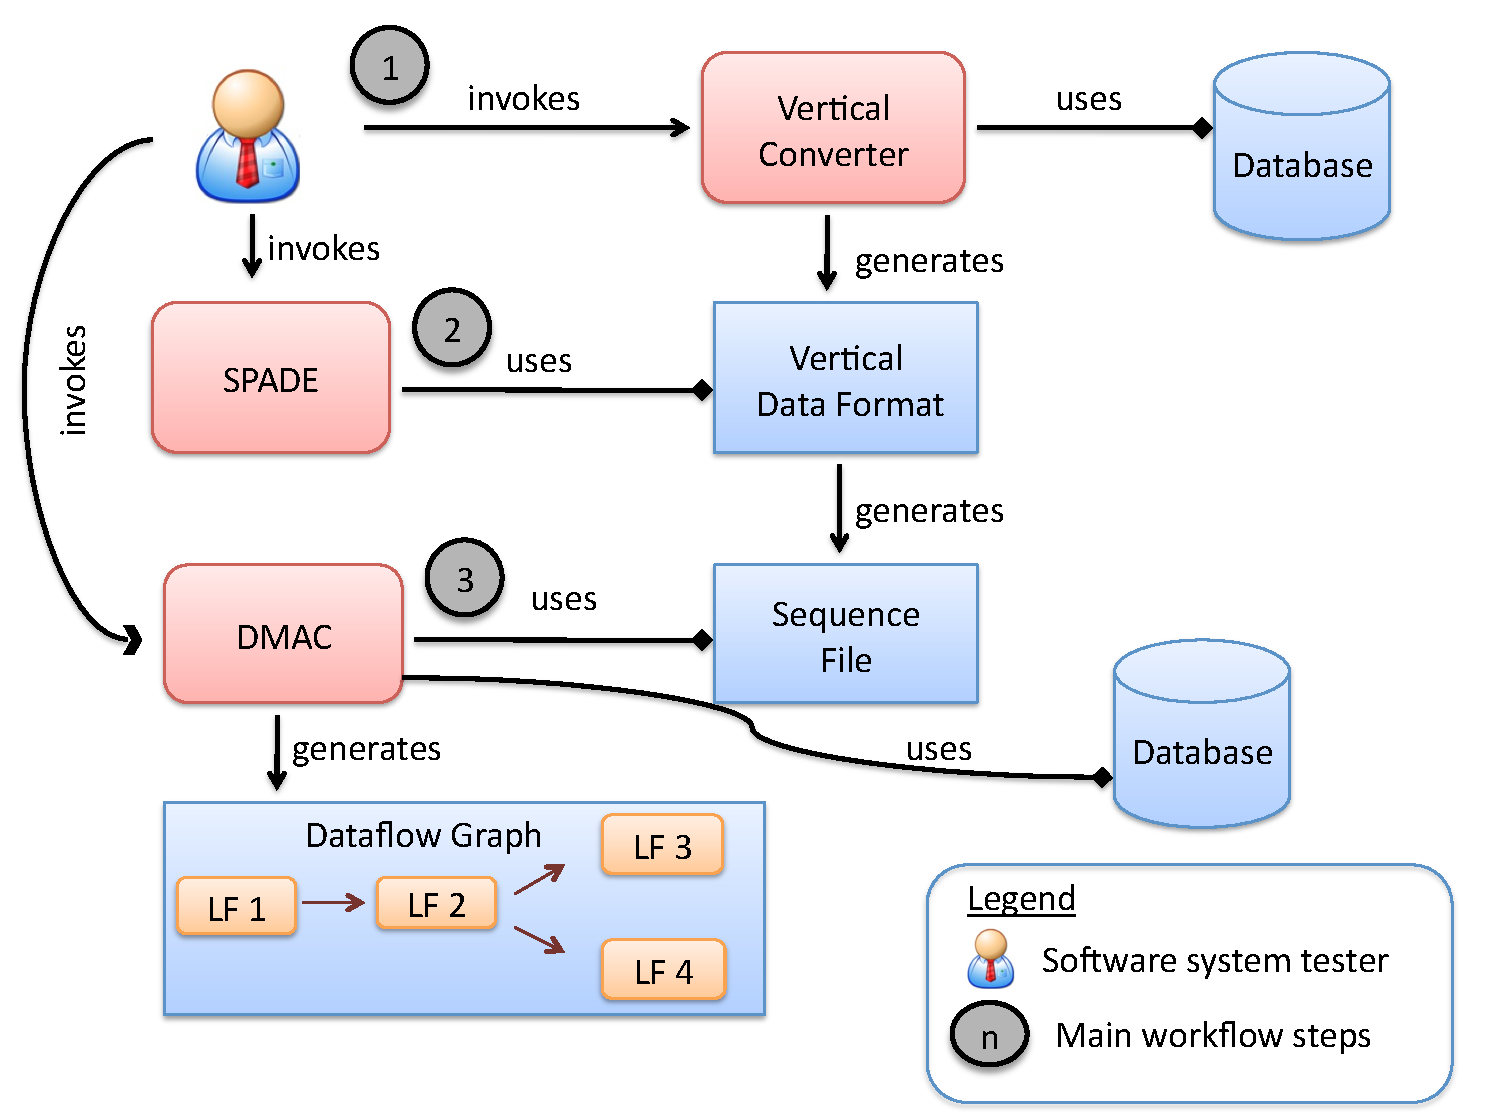
\includegraphics[scale=0.7]{analysis/dmac.pdf}
  \caption{Dataflow model auto-generation process.}
  \label{fig:dmac}
\end{figure}

\section{Process of auto constructing the dataflow model}
\label{sec:dmac-process}

This section describes different steps involved in auto constructing the 
dataflow model using DMAC.

\subsection{Finding frequently occurring word sequences}
\label{sec:frequent-mining}

As the first step frequent-sequence mining need to carried 
out to find out the frequently occurring word sequences 
in the system execution trace.

In data mining, frequent-sequence mining is the process of 
identifying frequently occurring sequences in a 
collection of time-stamped event-set such as purchased items 
in a transaction database. For example a \textit{customer-sequence} consists 
of a sequence of all transactions related to a particular 
customer. Customer-sequences are normally sorted on increasing 
transaction time. Finally, a customer-sequence supports a sequence 
$s$ if $s$ is a sub-sequence of that particular 
customer-sequence. 

To identify frequently occurring sequences, users have to 
supply a minimum number of customer-sequences. This is called 
\textit{minimum support} denoted by \textit{min-sup}. 
For a given database frequent-sequence mining locates sub-sequences 
that occur more than \textit{min-sup} customer-sequences.

In the context of system execution traces, we consider a 
customer-sequence an execution trace that consists of words. 
By words, we mean the items that can be separated by a delimiter 
(\textit{e.g.}, space and new-line). 

DMAC uses SPADE (\url{http://www.cs.rpi.edu/~zaki/www-new/pmwiki.php/Software/Software}) 
sequence mining tool to find out the frequently occurring word sequences. 

\begin{table}[h]
 \centering
 \caption{Sample system execution trace.}
 \label{table:trace1}
 \begin{tabular}{lccl}
 \hline
 \textbf{SID} & \textbf{message} \\
 \hline
 1 & A sent message 1 at 10.00 \\
 2 & A received message 1 at 10.01 \\
 \end{tabular}
\end{table}

\begin{table}[h]
 \centering
 \caption{Vertical data format for the system execution trace.}
 \label{table:trace-v-format}
 \begin{tabular}{lcccl}
 \hline
 \textbf{SID} & \textbf{EID} & \textbf{Size} & \textbf{Items} \\
 \hline
 1 & 1 & 1 & A \\ 
 1 & 2 & 1 & sent \\
 1 & 3 & 1 & message \\
 1 & 4 & 1 & 1 \\
 1 & 5 & 1 & at \\
 1 & 6 & 1 & 10.01 \\
 2 & 1 & 1 & A \\ 
 2 & 2 & 1 & received \\
 2 & 3 & 1 & message \\
 2 & 4 & 1 & 1 \\
 2 & 5 & 1 & at \\
 2 & 6 & 1 & 10.01 \\
 \end{tabular}
\end{table}

\textit{SPADE} requires data to be in a format called 
\textit{vertical id-list}. Table~\ref{table:trace1} contains 
two sample messages with a \texttt{Sequence Id (SID)} and 
the actual message. The corresponding vertical id-list for
the system execution trace in Table~\ref{table:trace1} is 
shown in the Table~\ref{table:trace-v-format}.  In addition 
to the \texttt{SID}, Table~\ref{table:trace-v-format} contains 
\texttt{Event ID (EID)}, which serves as a timestamp within
the sequence, and a \texttt{Size} field, which denotes how
many items are in the current transaction. In the context of 
a system execution trace, the \texttt{EID} is a monotonically 
increasing value and the \texttt{Size} is always one. Finally,
a word is considered as an item set and there is always just
one item in any transaction. 

DMAC has a tool called \textit{cuts-dmac-vertical} to convert the 
system execution trace into \textit{vertical id-list}.
Assuming the CUTS runtime architecture has been built 
and installed correctly, the CUTS DMAC vertical converter 
tool is installed at the following location:
\begin{lstlisting}
%> $CUTS_ROOT/bin/cuts-dmac-vertical
\end{lstlisting}
To see a complete list of command-line options, use the following 
command:
\begin{lstlisting}
%> $CUTS_ROOT/bin/cuts-dmac-vertical --help
\end{lstlisting}

Giving the database file as the input \textit{cuts-dmac-vertical} will 
convert the system execution trace into a vertical id-list ,which can be 
redirect into a file ending with \texttt{.data} extension 
as follows.
\begin{lstlisting}
%> $CUTS_ROOT/bin/cuts-dmac-vertical -f example.cdb > example.data
\end{lstlisting}

The next step is finding the frequently occurring word sequence using the 
\textit{SPADE} data mining tool. DMAC uses the version of \textit{SPADE} 
comes with the \textit{Data Mining Template Library (DMTL)}
(\url{http://sourceforge.net/projects/dmtl/}) data mining tool. 
DMTL can be downloaded from the following location
\url{http://sourceforge.net/projects/dmtl/} . 
After extracting the DMTL distribution change, to the directory named \textit{test} 
inside the distribution and use the following command to to find out 
the command line options.
\begin{lstlisting}
%> $DMTL_INSTALL_DIR/test/sequence_test -h
\end{lstlisting}

To find out the frequent-sequences which have a equal or 
higher occurrence than the provided \textit{min-sup} value, 
SPADE can be executed providing the \textit{min-sup} value and the vertical-id 
list of the system execution trace as follows.
\begin{lstlisting}
%> $DMTL_ROOT/test/sequence_test -i example.data -s 100 -p > example-sequence
\end{lstlisting}

The \texttt{-i} option specifies the vertical-id list created in the previous step, 
\texttt{-s} option specifies the \textit{min-sup} value and \textit{-p} option 
specifies the output to be printed to the standard input. In the above case 
the output is redirected to a file called \textit{example-sequence}. This file 
is fed to DMAC to generate the dataflow model in the next step.

\subsection{Auto generating the dataflow model}
\label{sec:auto-generating}

Having find out the frequent-sequences of a particular system 
execution trace the next step is to generate the dataflow model which 
has log formats and cause-effect relations. This step is done using a tool called 
\textit{cuts-dmac}.

Assuming the CUTS runtime architecture has been built 
and installed correctly, the \textit{cuts-dmac} tool is installed at the 
following location:
\begin{lstlisting}
%> $CUTS_ROOT/bin/cuts-dmac
\end{lstlisting}
To see a complete list of command-line options, use the following 
command:
\begin{lstlisting}
%> $CUTS_ROOT/bin/cuts-dmac-vertical --help
\end{lstlisting}

Using the system execution trace and the frequent-sequence 
file (eg: example-sequence) generated in the previous step, following 
is how to generate the dataflow model for the given system execution 
trace.

\begin{lstlisting}
%> $CUTS_ROOT/bin/cuts-dmac -i example-sequence -f example.cdb -n example
\end{lstlisting}

This will output the possible log formats and relations which will be useful for 
QoS analysis. Further it will create a datagraph file using the argument 
provided for \texttt{-n}. For the abobve invocation it will create a datagraph 
file named \textit{example.datagraph}. This datgraph contains all the 
possible log formats and the cause-effect relations among them based on 
the frequent-sequence mining. Distributed system testers can prune this 
datagraph file further to find out the QoS 
properties depending on the scenario been analyzed. The above invocation 
also output the coverage (as a percentage) of each log format in the system 
execution trace. This is to assist distributed system testers to take decisions 
on pruning the generated datagraph file.